\section{Interaktion der Komponenten}
Auf Basis der Use Cases aus der Analyse wird in diesem Kapitel die Interaktion der einzelnen Komponenten aus Kapitel 1 betrachtet. 
Dabei liegt der Fokus vor allem auf der Interaktion zwischen der RobotUnit und dem Server, wie dessen Austausch mit dem Hospital und der Taxiapp. 
Die Abläufe innerhalb der Komponenten werden dann in Kapitel 8 näher spezifiziert. \\


\subsection*{Interaktion bei Ausführung von \emph{Receive Order \& Cancel Order}}

Elementar ist in diesem Fall der Use Case "ReceiveOrder" (Use Case 1.1), der es Usern ermöglicht Anfragen oder Notrufe abzusetzen, um ein Taxi oder einen Krankentransporter anzufordern. 
Das System arbeitet mit einer Warteliste. 
Krankentransporte werden in jedem Fall priorisiert und es wird schnellstmöglich der nächste Robot zur Verfügung gestellt. 
Im Falle des ersten Sequenzdiagramms ist dies mit der Verwendung der TaxiApp dargestellt, die wiederum den Task mit den Destinations an den Server weitergibt. 
Danach wird vom Server überprüft, ob überhaupt Taxis verfügbar sind.
Falls keins mehr verfügbar ist, wird die Anzahl der Kunden in der Wartschlange an die App und somit an den User zurückgegeben. 
Mit "Cancel Order" (Use Case 1.2) können sich User dabei aus der Warteliste streichen lassen, solange sie noch nicht in das Taxi eingestiegen sind. \\

\begin{figure}[H]
	\centering
	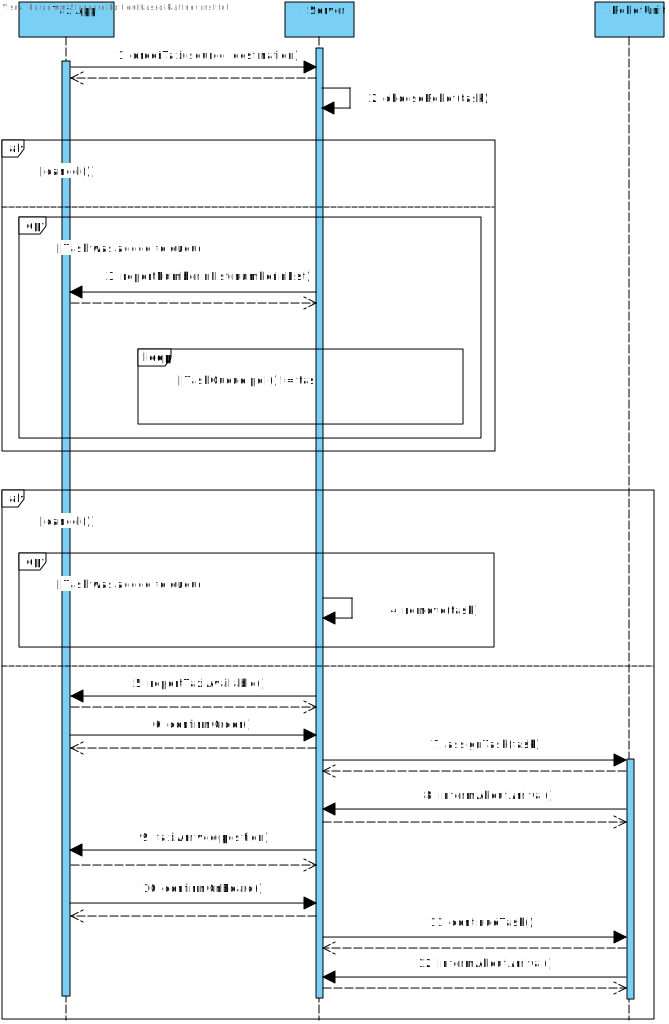
\includegraphics[width=0.9\textwidth]{img/2-Entwurf-ReceiveOrder-Taxi}
	\caption{\emph{ReceiveOrder}-Sequenzdiagramm, falls ein Kunde ein Taxi anfragt}
	\label{SequenzDiagrammInteraktion}
\end{figure}

\begin{figure}[H]
	\centering
	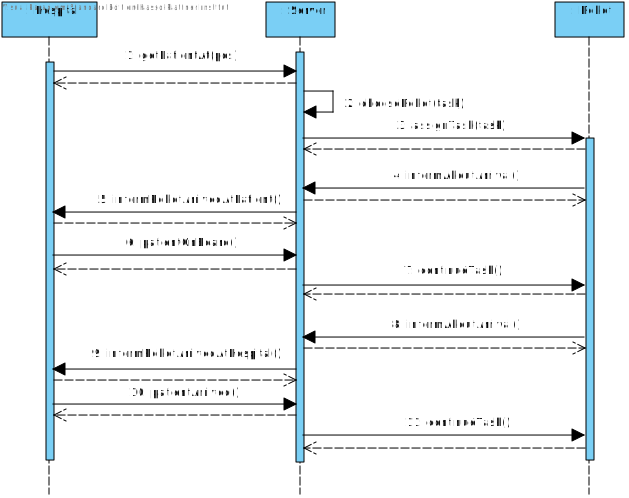
\includegraphics[width=0.9\textwidth]{img/2-Entwurf-ReceiveOrder-Hosp}
	\caption{\emph{RecieveOrder}-Sequenzdiagramm, falls das Hospital einen neuen Patienten meldet}
	\label{SequenzDiagrammInteraktion}
\end{figure}



\subsection*{Interaktion bei Ausführung von \emph{Receive Boarding Confirmation \& Receive Arrival Notification}}

Alle Prozesse laufen wie ersichtlich über den Server, der wiederum die RobotUnit fernsteuert. 
So wird für "Receive Boarding Confirmation" (Use Case 1.3) erst vom Hospital oder der TaxiApp an den Server zurückgemeldet, dass sich der Patient oder der Customer an Bord befindet, bevor die Fahrt aufgenommen werden kann. 
In gleicher Weise wird dem Server mit "Receive Arrival Notification" (Use Case 1.5) zurückgemeldet, dass der Robot wieder für weitere Einsätze verfügbar ist, sobald der Customer den Robot verlassen hat.  \\

\begin{figure}[H]
	\centering
	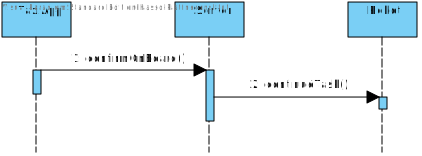
\includegraphics[width=0.9\textwidth]{img/2-Entwurf-ReceiveBoardingConfirmation-taxi}
	\caption{\emph{ReceiveBoardingConfirmation-taxi}-Sequenzdiagramm}
	\label{SequenzDiagrammInteraktion}
\end{figure}

\begin{figure}[H]
	\centering
	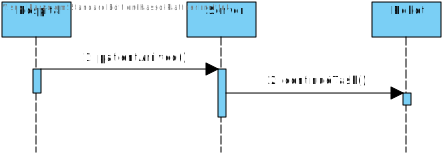
\includegraphics[width=0.9\textwidth]{img/2-Entwurf-ReceiveUnloadConfirmation-hospital}
	\caption{\emph{ReceiveUnloadConfirmation-hospital}-Sequenzdiagramm}
	\label{SequenzDiagrammInteraktion}
\end{figure}


\subsection*{Interaktion bei Ausführung von \emph{Use Cases Perfom Task \& Continue Task}}
Konkret wird der RobotUnit dabei über die Use Cases "Perfom Task" (Use Case 2.2) und "Continue Task" (Use Case 2.3) ein Task zugewiesen, der solange ausgeführt wird, bis der Task abgebrochen wird oder das Ziel erfolgreich erreicht wurde und dies an den Server zurückgemeldet werden kann. \\

\begin{figure}[H]
	\centering
	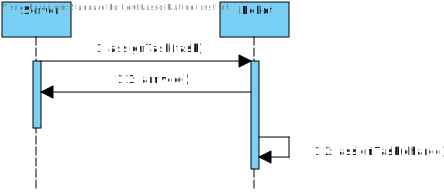
\includegraphics[width=0.9\textwidth]{img/2-Entwurf-PerformTask}
	\caption{\emph{Perform Task}-Sequenzdiagramm}
	\label{SequenzDiagrammInteraktion}
\end{figure}

Die weiteren Use Cases sind diesen untergeordnet; enthalten entweder nur einseitige Server/RobotUnit Kommunikation, wie zum Beispiel bei "Request Repair" (Use Case 1.6) oder haben ihren Fokus vor allem auf den Wechselwirkungen innerhalb der RobotUnit (Siehe dazu Kapitel 8). \\

